%! Author = Stepan Oskin
%! Date = 09-Jul-19

% Preamble
\documentclass[11pt]{article}
% Packages
\usepackage{amsmath, subcaption}
\usepackage{graphicx}

% New commands
\newcommand{\norm}[1]{\left\lVert#1\right\rVert}
\newcommand{\vect}[1]{\boldsymbol{#1}}
% Document
\begin{document}

    \title{Mathematics of Support Vector Machines (SVM) \\
    Excerpts from Python Machine Learning \\
    Second Edition \\
    By Sebastian Raschka and Vahid Mirjalili \\
    and other sources}

    \author{Stepan Oskin}

    \maketitle

    \begin{abstract}

        Support Vector Machines (SVM) are a family of powerful and widely used learning algorithms,
        which can be considered an extension of the perceptron.
        Given a set of training examples, each marked as belonging to one or the other of two categories,
        an SVM training algorithm builds a model that assigns new examples to one category or the other,
        making it a non-probabilistic binary linear classifier (although methods exist to use SVM in
        a probabilistic classification setting).
        While in perceptron, the optimization objective is to minimize misclassification errors,
        in SVMs the learning objective is to maximize the margin.
        The margin is defined as the distance between the separating hyperplane (decision boundary)
        and the training samples that are closest to this hyperplane, which are the so-called support vectors.
        In addition to performing linear classification, SVMs can efficiently perform a non-linear classification
        using what is called the kernel trick, implicitly mapping their inputs into high-dimensional feature spaces.

    \end{abstract}

    \section{Classification} \label{sec:classification}

    Classifying data is a common task in machine learning.
    Suppose some given data points each belong to one of two classes, and the goal is to decide which class a
    new data point will be in.
    In the case of support-vector machines, a data point is viewed as a $p$-dimensional vector
    (a list of $p$ numbers), and we want to know whether we can separate such points with
    a $(p-1)$-dimensional hyperplane.
    This is called a linear classifier.
    There are many hyperplanes that might classify the data.
    One reasonable choice as the best hyperplane is the one that represents the largest separation, or margin,
    between the two classes.
    So we choose the hyperplane so that the distance from it to the nearest data point on each side is maximized.
    If such a hyperplane exists, it is known as the \textbf{maximum-margin hyperplane} and the linear classifier it defines
    is known as a \textbf{maximum-margin classifier};
    or equivalently, the perceptron of optimal stability.

    \section{Maximum margin classification with support vector machines} \label{sec:max_marg_class}

    Support Vector Machine (SVM) is a powerful and widely used learning algorithm, which can be considered
    an extension of the perceptron.
    For perceptron algorithm, optimization objective is to minimize misclassification errors.
    However, in SVMs the optimization objective is to \textbf{maximize the margin}.
    The margin is defined as the \textbf{distance between the separating hyperplane (decision boundary) and the training
    samples} that are closest to this hyperplane, which are the so-called \textbf{support vectors}.
    This is illustrated in figure~\ref{fig:svm}:

    \begin{figure}[hbt!]
        \centering
        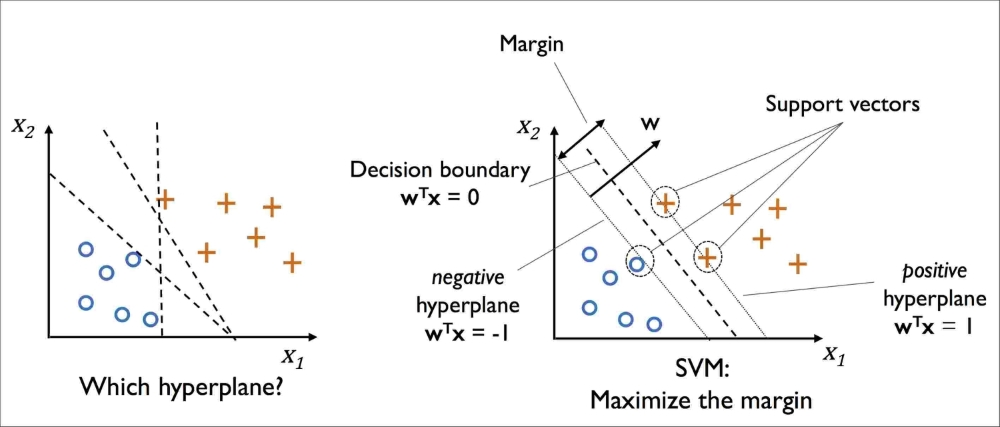
\includegraphics[width=1\linewidth,trim=4 4 4 4,clip]{img/svm.jpg}
        \caption{Optimization objective in Support Vector Machines is to maximize the margin between the training samples
        that are closest to the hyperplane (decision boundary).}
        \label{fig:svm}
    \end{figure}

    An SVM model is a representation of the examples as points in space, mapped so that the examples of the separate
    categories are divided by a clear gap that is as wide as possible.
    New examples are then mapped into that same space and predicted to belong to a category based on which side of
    the gap they fall.

    \section{Maximum margin intuition} \label{sec:max_marg_int}

    The rationale behind having decision boundaries with large margins is that they tend to have a lower
    generalization error whereas models with small margins are more prone to overfitting.
    To get an idea of the margin maximization, let's take a closer look at those positive and
    negative hyperplanes that are parallel to the decision boundary, which can be expressed as follows:

    \begin{equation}
        \label{eq:pos_hyp}
        w_0 + \vect{w}^T \vect{x}_{pos} = 1
    \end{equation}

    \begin{equation}
        \label{eq:neg_hyp}
        w_0 + \vect{w}^T \vect{x}_{neg} = -1
    \end{equation}

    If we subtract those two linear equations~\ref{eq:pos_hyp} and~\ref{eq:neg_hyp} from each other, we get:

    \begin{equation}
        \label{eq:pos-neg}
        \implies \vect{w}^T (\vect{x}_{pos} - \vect{x}_{neg}) = 2
    \end{equation}

    We can normalize this equation (\ref{eq:pos-neg}) by the length of the vector $\vect{w}$, which is defined as follows:

    \begin{equation}
        \label{eq:vect_norm}
        \norm{ \vect{w} } = \sqrt{ \sum \limits_{j=1}^m w_j^2 }
    \end{equation}

    So we arrive at the following equation:

    \begin{equation}
        \label{eq:pos-neg_norm}
        \large{
        \frac{ \vect{w}^T ( \vect{x}_{pos} - \vect{x}_{neg} ) } { \norm{ \vect{w} } }
        = \frac{2} { \norm{ \boldsymbol{w} } }
        }
    \end{equation}

    The left side of the preceding equation can then be interpreted as the \textbf{distance between the positive
    and negative hyperplane}, which is the so-called \textbf{margin} that we want to maximize.

    Now, the \textbf{objective function} of the SVM becomes the \textbf{maximization of this margin} by maximizing
    \begin{equation}
        \label{eq:svm_margin}
        \frac{2} {\norm{\vect{w}}}
    \end{equation}
    under the \textbf{constraint} that the samples are classified correctly, which can be written as:

    \begin{equation}
        \label{eq:svm_constraints}
        \begin{gathered}
            w_0 + \vect{w}^T \vect{x}^{(i)} \geq 1 \text{ if } y^{(i)} = 1 \\
            w_0 + \vect{w}^T \vect{x}^{(i)} \leq 1 \text{ if } y^{(i)} = -1 \\
            \text{for } i=1 \dots N
        \end{gathered}
    \end{equation}


    Here, \textbf{N} is the number of samples in our dataset.

    These two equations basically say that \textbf{all negative samples should fall on one side of the negative hyperplane,
    whereas all the positive samples should fall behind the positive hyperplane}, which \textbf{can also be written more
    compactly} as follows:

    \begin{equation}
        \label{eq:svm_cons_comp}
        y^{(i)} \left( w_0 + \vect{w}^T \vect{x}^{(i)} \right) \geq 1 ~ \forall_i
    \end{equation}

    In practice though, it is easier to minimize the \textbf{reciprocal term}:
    \begin{equation}
        \label{eq:svm_margin_reciprocal}
        \frac{1} {2} \norm{\vect{w}}^2
    \end{equation}
    which can be solved by quadratic programming.

    \section{Dealing with a non-linearly separable case using slack variables} \label{sec:slack_vars}

    Although we don't want to dive much deeper into the more involved mathematical concepts behind the maximum-margin
    classification, let us briefly mention the slack variable $\xi$ , which was introduced by Vladimir Vapnik in
    1995 and led to the so-called \textbf{soft-margin classification}.
    The motivation for introducing the slack variable $\xi$ was that the linear constraints need to be relaxed for
    non-linearly separable data to allow the convergence of the optimization in the presence of misclassifications,
    under appropriate cost penalization.

    The positive-values slack variable is simply added to the linear constraints:

    \begin{equation}
        \label{eq:svm_constraints_slack}
        \begin{gathered}
            w_0 + \boldsymbol{w}^T \boldsymbol{x}^{(i)} \geq 1 - \xi^{(i)} \text{ if } y^{(i)} = 1 \\
            w_0 + \boldsymbol{w}^T \boldsymbol{x}^{(i)} \leq - 1 + \xi^{(i)} \text{ if } y^{(i)} = -1 \\
            \text{for } i=1 \dots N
        \end{gathered}
    \end{equation}

    Here, \textbf{N} is the number of samples in our dataset.
    So the new objective to be minimized (subject to the constraints) becomes:

    \begin{equation}
        \label{eq:svm_margin_reciprocal_slack}
        \frac{1} {2} \norm{\vect{w}}^2 + C \left( \sum \limits_i \xi^{(i)} \right)
    \end{equation}

    Via the variable \texttt{C}, we can then control the penalty for misclassification.

    Large values of \texttt{C} correspond to large error penalties, whereas we are less strict about
    misclassification errors if we choose smaller values for \texttt{C}.
    We can then use the \texttt{C} parameter to control the width of the margin and therefore tune the
    bias-variance trade-off, as illustrated in the figure~\ref{fig:svm_c}:

    \begin{figure}[hbt!]
        \centering
        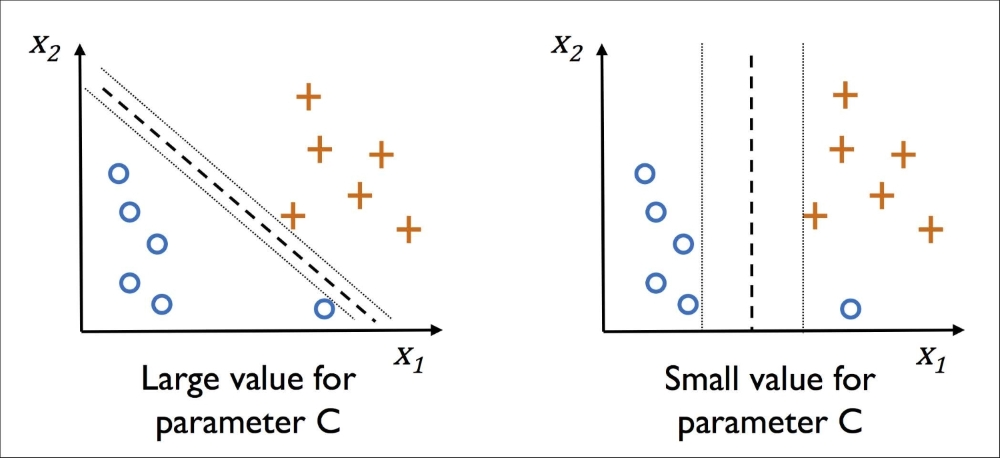
\includegraphics[width=1\linewidth,trim=4 4 4 4,clip]{img/svm_c.jpg}
        \caption{In Support Vector Machines, penalty for misclassification can be controlled by adjusting the values
        of parameter C. Large values of C correspond to large error penalties, whereas smaller values treat
        misclassifications less strictly.}
        \label{fig:svm_c}
    \end{figure}

    This concept is related to regularization, which is discussed in the document covering Logistic Regression,
    in the context of regularized regression where decreasing the value of \texttt{C} increases the bias and lowers the
    variance of the model.

    The three decision regions of the SVM, visualized after training the classifier on the Iris flower dataset, are presented on figure~\ref{fig:iris_svm_linear}.

    \begin{figure}[hbt!]
        \centering
        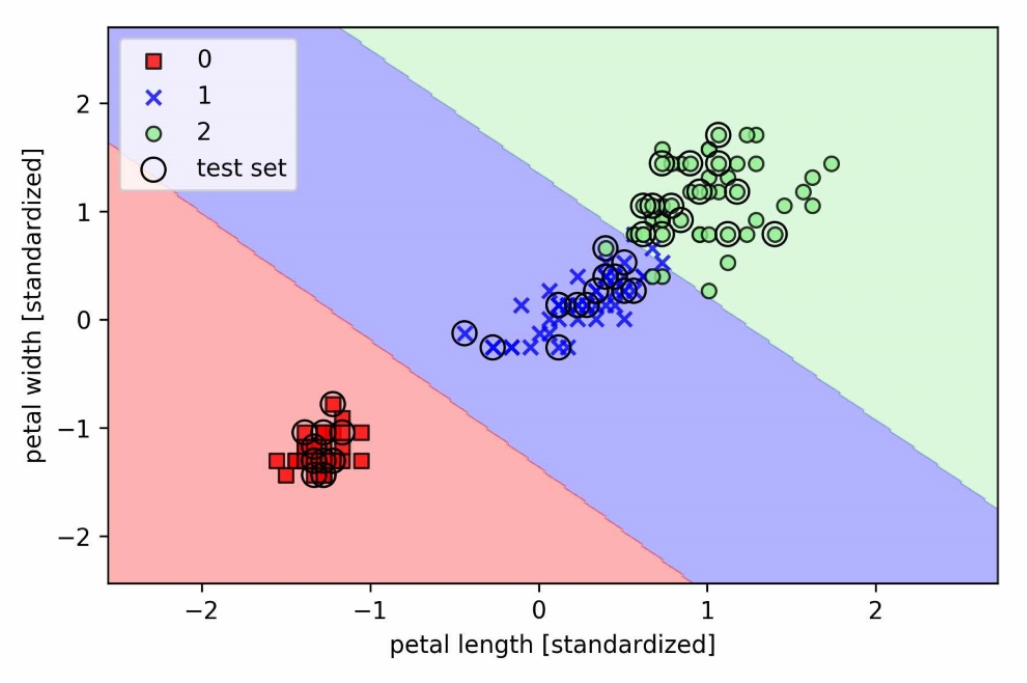
\includegraphics[width=1\linewidth,trim=4 4 4 4,clip]{img/iris_svm_linear.png}
        \caption{The three decision regions of the linear SVM after training the classifier on the Iris flower dataset.
        Results of SVM are similar to those yielded by a Logistic Regression model.}
        \label{fig:iris_svm_linear}
    \end{figure}

    \section{Logistic regression versus support vector machines} \label{sec:log_reg_vs_svm}

    In practical classification tasks, linear logistic regression and linear SVMs often yield very similar results.
    Logistic regression tries to maximize the conditional likelihoods of the training data, which makes it more prone to outliers than SVMs, which mostly care about the points that are closest to the decision boundary (support vectors).
    On the other hand, logistic regression has the advantage that it is a simpler model and can be implemented more easily.
    Furthermore, logistic regression models can be easily updated, which is attractive when working with streaming data.

    \section{SVM implementations in \texttt{scikit-learn}}\label{sec:svm_sklearn}

    For practical purposes, it is better to use \texttt{scikit-learn}'s more optimized implementation of SVM that also supports multi-class settings off the shelf (OvR by default).
    The \texttt{scikit-learn} library's \texttt{Perceptron} and \texttt{LogisticRegression} classes make use of the \textit{LIBLINEAR} library, which is a highly optimized C/C++ library developed at the National Taiwan University\cite{Fan2008}.
    Similarly, the \texttt{SVC} class that we used to train an SVM makes use of \textit{LIBSVM} library, which is an equivalent C/C++ library specialized for SVMs\cite{Chang2001}.

    The advantage of using LIBLINEAR and LIBSVM over native Python implementations is that they allow the extremely quick training of large amounts of linear classifiers.
    However, sometimes our datasets are too large to fit into computer memory.
    Thus, \texttt{scikit-learn} also offers alternative implementations via the \texttt{SGDClassifier} class, which also supports online learning via the \texttt{partial\_fit} method.
    The concept behind the \texttt{SGDClassifier} class is similar to the stochastic gradient algorithm that we implemented for Adaline.

    \section{Kernel methods for linearly inseparable data} \label{sec:kernel}

    \begin{figure}[hbt!]
        \centering
        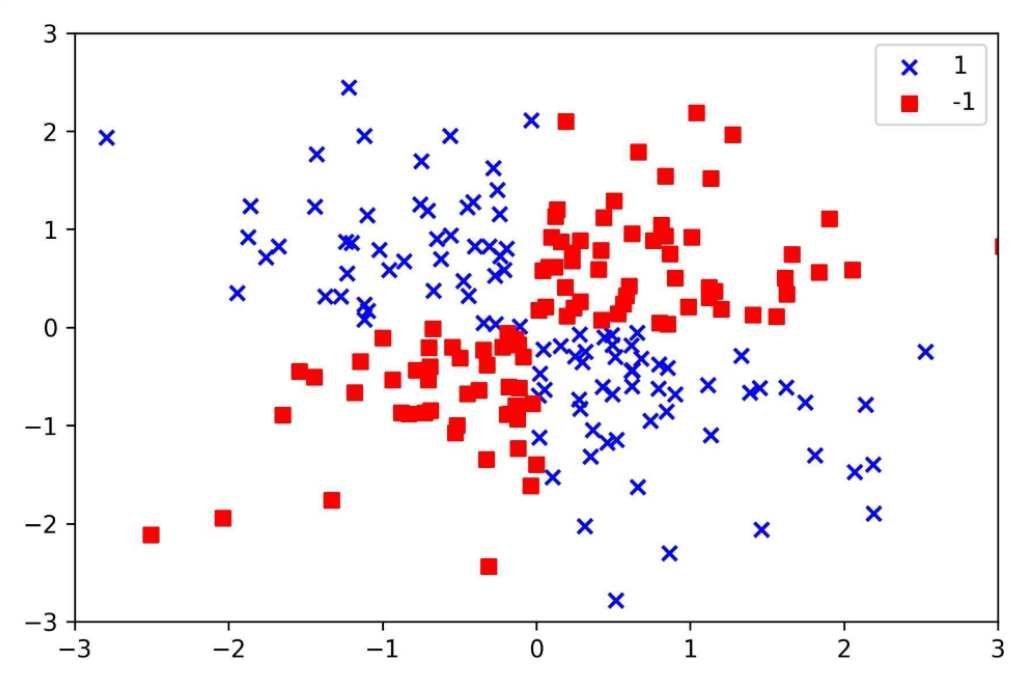
\includegraphics[width=1\linewidth,trim=4 4 4 4,clip]{img/non_lin_data.png}
        \caption{Sample dataset generated in a form of a XOR gate, where 100 samples are assigned the class label 1, and 100 samples are assigned class label -1.
        In this dataset, samples from positive and negative classes cannot be separated well using a linear hyperplane as a decision boundary.}
        \label{fig:non_lin_data}
    \end{figure}

    Another reason why SVMs enjoy high popularity among machine learning practitioners is that it can be easily \textbf{kernelized} to solve nonlinear classification problems.
    On figure~\ref{fig:non_lin_data} we can see an example of a nonlinear classification problem.
    This dataset was randomly generated using \texttt{NumPy} library in Python;
    it consists of 100 samples of class 1 and 100 samples of class -1, and has a form of a XOR gate.

    Obviously, we would not be able to separate samples from the
    positive and negative class very well using a linear hyperplane
    as a decision boundary via the linear logistic regression or
    linear SVM model that we discussed in earlier sections.

    \section{The basic idea behind kernel methods} \label{sec:kern_idea}

    \begin{figure}[hbt!]
        \centering
        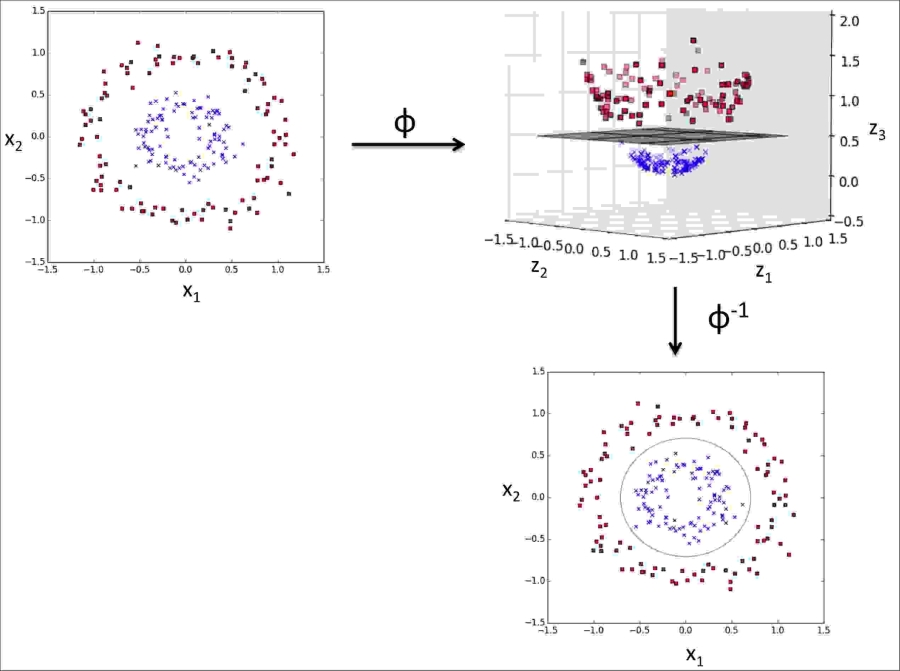
\includegraphics[width=1\linewidth,trim=4 4 4 4,clip]{img/kernel.jpg}
        \caption{An example of a linearly inseparable two-dimensional dataset being transformed via a mapping function $\phi$ onto a three-dimensional space, where it becomes linearly separable, and then re-projected back to the two-dimensional space.
        This transformation represents the basic idea behind kernel methods.}
        \label{fig:kernel}
    \end{figure}

    The basic idea behind \textbf{kernel methods} to deal with such linearly inseparable data is to create nonlinear combinations of the original features to project them onto a higher-dimensional space via a mapping function $\phi$ where it becomes linearly separable.
    As shown in figure~\ref{fig:kernel}, we can transform a two-dimensional dataset onto a new three-dimensional feature space where the classes become separable via the following projection:

    \begin{equation}
        \label{eq:kern_ex}
        \phi(x_1, x_2) = (z_1, z_2, z_3) = (x_1, x_2, x_1^2 + x_2^2)
    \end{equation}

    This allows us to separate the two classes shown in the plot via a linear hyperplane that becomes a nonlinear decision boundary if we project it back onto the original feature space:

    \section{Using the kernel trick to find separating hyperplanes in high-dimensional space}\label{sec:kernel_trick}

    To solve a nonlinear problem using an SVM, we would transform the training data onto a higher-dimensional feature space via a mapping function $\phi$ and train a linear SVM model to classify the data in this new feature space.
    Then, we can use the same mapping function to transform new, unseen data to classify it using the linear SVM model.

    However, one problem with this mapping approach is that the construction of the new features is computationally very expensive, especially if we are dealing with high-dimensional data.
    This is where the so-called \textbf{kernel trick} comes into play.
    Although we didn't go into much detail about how to solve the quadratic programming task to train an SVM, in practice all we need is to replace the dot product $\vect{x}^{(i)T}\vect{x}^{(j)}$ by $ \phi \left( \vect{x}^{(i)} \right)^T \phi \left( \vect{x}^{(j)} \right) $.
    In order to save the expensive step of calculating this dot product between two points explicitly, we define a so-called \textbf{kernel function}:

    \begin{equation}
        \label{eq:kernel_func}
        \kappa \left( \boldsymbol{x}^{(i)}, \boldsymbol{x}^{(j)} \right) & = \phi \left( \boldsymbol{x}^{(i)} \right)^T \phi \left( \boldsymbol{x}^{(j)} \right)
    \end{equation}


    One of the most widely used kernels is the \textbf{Radial Basis Function (RBF)} kernel or simply called the \textbf{Gaussian kernel}:

    \begin{equation}
        \label{eq:kernel_rbf}
        \large{
        \kappa ( \vect{x}^{(i)}, \vect{x}^{(j)} )
        & = \exp \left( - \frac{ \norm{ \vect{x}^{(i)} - \vect{x}^{(j)} }^2} {2 \sigma ^2} \right)
        }
    \end{equation}

    This is often simplified to:

    \begin{equation}
        \label{eq:kernel_rbf_simple}
        \large{
        \kappa( \vect{x}^{(i)}, \vect{x}^{(j)} )
        & = \exp \left( - \gamma \norm{ \vect{x}^{(i)} - \vect{x}^{(j)} } ^2 \right) }
    \end{equation}

    Here, $\large{\gamma = \frac{1} {2 \sigma^2}}$ is a free parameter that is to be optimized.

    Roughly speaking, the term \textbf{kernel} can be interpreted as a \textbf{similarity function} between a pair of samples.
    The \textbf{minus sign inverts the distance measure into a similarity score}, and, due to the exponential term, the resulting similarity score will fall into a range between 1 (for exactly similar samples) and 0 (for very dissimilar samples).

    Now that we defined the big picture behind the kernel trick, let us see if we can train a kernel SVM that is able to draw a nonlinear decision boundary that separates the XOR data well.
    Here, we simply use the \texttt{SVC} class from \texttt{scikit-learn} that and replace the \texttt{kernel='linear'} parameter with \texttt{`kernel='rbf'}.
    As we can see in the resulting plot on figure~\ref{fig:non_lin_data_svm}, the kernel SVM separates the XOR data relatively well:

    \begin{figure}[hbt!]
        \centering
        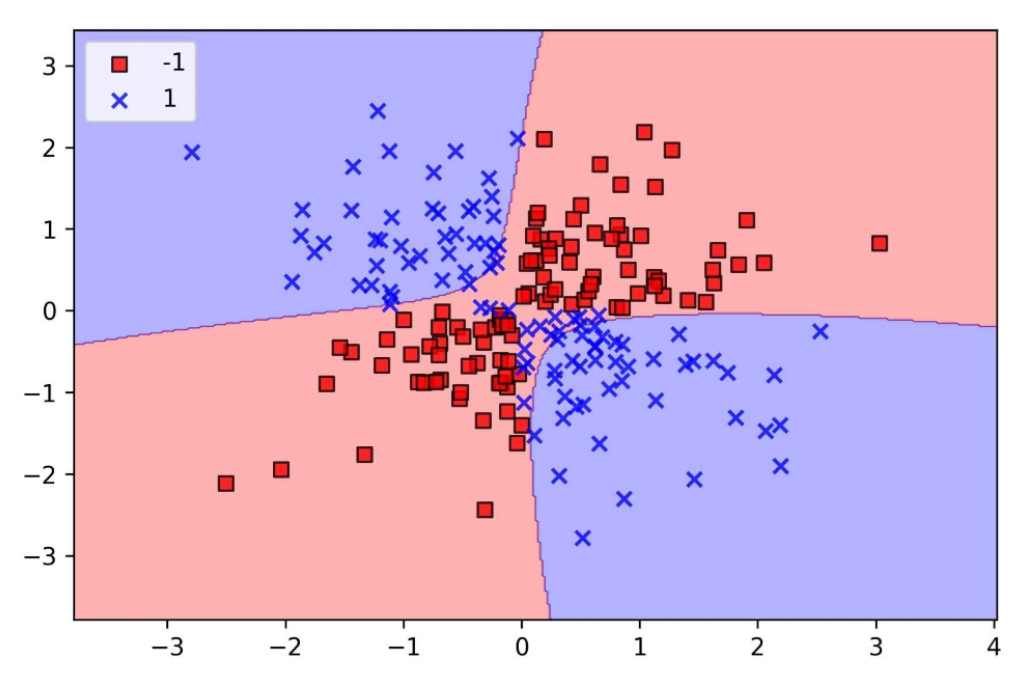
\includegraphics[width=1\linewidth,trim=4 4 4 4,clip]{img/non_lin_data_svm.png}
        \caption{Nonlinear decision boundary drawn by a kernel SVM is separating the XOR data relatively well.
        Cut-off parameter $\gamma$ was set to 0.1.}
        \label{fig:non_lin_data_svm}
    \end{figure}

    \section{Cut-off parameter $\gamma$ for the Gaussian sphere} \label{sec:gamma}

    The $\gamma$ parameter, which was set to \texttt{gamma=0.1} in the example with XOR data, can be understood as a \textbf{cut-off} parameter for the Gaussian sphere.
    If we increase the value for $\gamma$, we increase the influence or reach of the training samples, which leads to a tighter and bumpier decision boundary.
    To get a better intuition for $\gamma$, below on figure~\ref{fig:iris_svm_rbf} we present the two different values of $\gamma$ (0.2, and 100) applied to an RBF kernel SVM that was used to classify Iris flower dataset:

    \begin{figure}[hbt!]
        \centering
        \begin{subfigure}[t]{.48\textwidth}
            \centering
            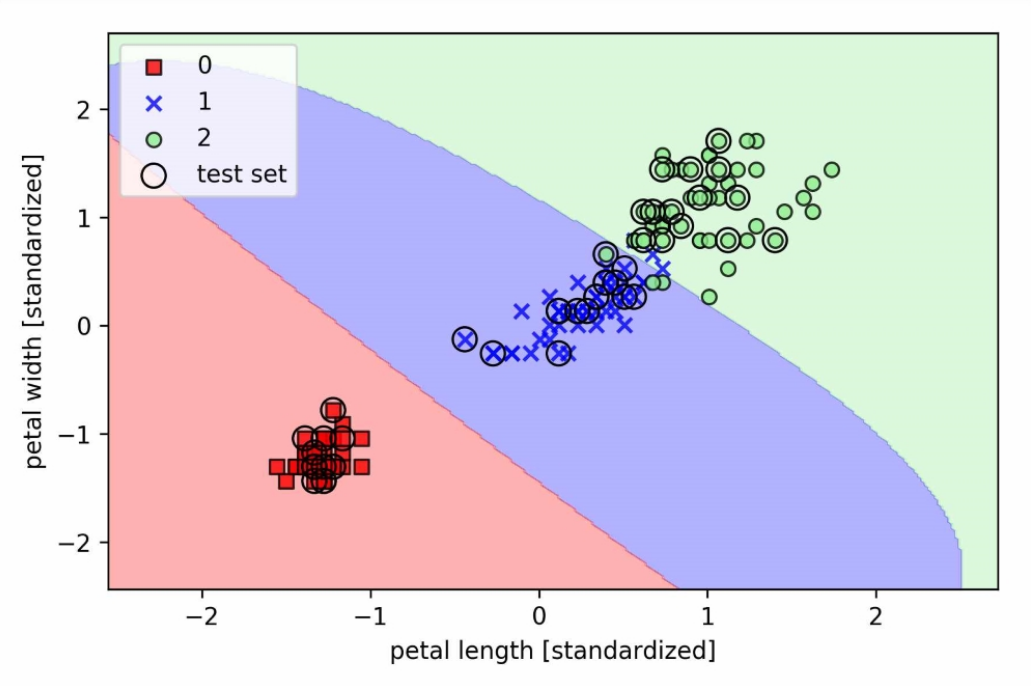
\includegraphics[width=\columnwidth]{img/iris_svm_gamma_02.png}
            \caption{$\gamma=0.2$}
            \label{fig:iris_svm_gamma_0.2}
        \end{subfigure}
        ~ %add desired spacing between images, e. g. ~, \quad, \qquad, \hfill etc.
        %(or a blank line to force the subfigure onto a new line)
        \begin{subfigure}[t]{.48\textwidth}
            \centering
            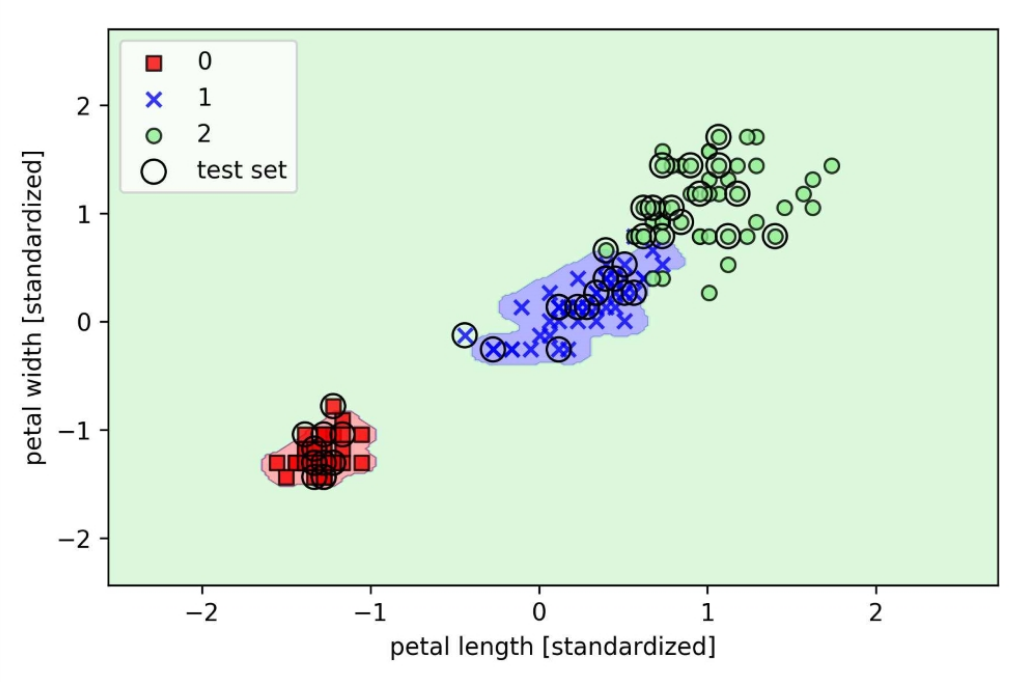
\includegraphics[width=\columnwidth]{img/iris_svm_gamma_100.png}
            \caption{$\gamma=100$}
            \label{fig:iris_svm_gamma_100}
        \end{subfigure}
        \caption{Different values of parameter $\gamma$ applied to an RBF kernel SVM that was used to classify Iris flower dataset.
        Large value of $\gamma$ (\ref{fig:iris_svm_gamma_100}) results in the model fitting the training dataset very well, but will likely have a high generalization error on unseen data.
        This illustrates that the $\gamma$ parameter also plays an important role in controlling overfitting.}
        \label{fig:iris_svm_rbf}
    \end{figure}

    If we choose a relatively small value for $\gamma$, the resulting decision boundary of the RBF kernel SVM model will be relatively soft, as shown in figure~\ref{fig:iris_svm_gamma_0.2}.
    When using a relatively large value of $\gamma$, the decision boundary around the classes 0 and 1 is much tighter, as can be seen in figure~\ref{fig:iris_svm_gamma_100}.
    Although the model fits the training dataset very well, such a classifier will likely result in a high generalization error on unseen data.
    This illustrates that the $\gamma$ parameter also plays an important role in controlling overfitting.

    \section{More information on SVM} \label{sec:svm_det}

    More detailed description of support vector machines can be found in \textit{The Nature of Statistical Learning Theory} book by Vladimir Vapnik\cite{Vapnik2000}, \textit{A Practical Guide to Support Vector Classification} tutorial from National Taiwan University\cite{Hsu2003}, or Chris J.C.\ Burges' excellent explanation in
    \textit{A Tutorial on Support Vector Machines for Pattern Recognition}~\cite{Burges1998}.

    \medskip
    \bibliography{svm}
    \bibliographystyle{ieeetr}

\end{document}